\documentclass[document.tex]{subfiles}
\begin{document}
\section*{Exercise 3:}

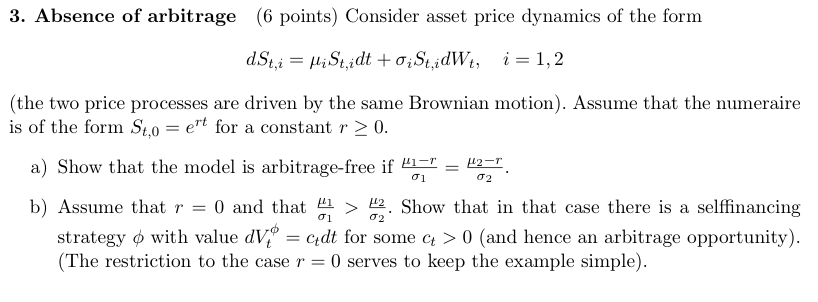
\includegraphics[width=\textwidth]{ex3.png}


We have 2 stocks who follow the following SDE:

\begin{equation}
d S^i_t = \mu S^i_t dt + \sigma S^i_t d W_t
\end{equation}

a) To show that the market is arbitrage free we have to show that the market admits an equivalent martingale measure. We will show this by finding one. \\

The discounted value process is a Q-martingale if and only if $S^1_t = S^1_0 + \int_0^t rS^1_s ds + M^Q_t$ with $M^Q_t$ being a Q-local martingale.

We define $\tilde{W_t} = W_t + \int_0^t  \frac{\mu - r}{\sigma} ds$ and use Girsanov to get Q under which $\tilde{W}$ is again a brownian motion.

\begin{equation}
\frac{d Q}{d P} = exp(-\frac{\mu_i - r}{\sigma_i} W_T - \frac{1}{2} (\frac{\mu_i - r}{\sigma_i})^2 T)
\end{equation}

As we can see the unique martingale measure only depends on $\frac{\mu_i - r}{\sigma_i}$. As this expression is equal for our two assets they are both martingales under Q. From the existence of a martingale measure it follows that there can be no arbitrage. \\ \\

b) In the given example the market value of risk is higher for the second asset. Intuitively both assets move together due to brownian motion that drives both processes. But asset 1 has a higher drift. This means for our strategy we buy asset 1 and sell asset 2. We assume $S_{0, 1} = S_{0, 2}$ and buy $\frac{1}{\sigma_1}$ of asset 1 and sell $\frac{1}{\sigma_2}$ units of asset 2. Then we get:

\begin{equation}
d V_t^{\phi} = \frac{1}{\sigma_1} d S_{t, 1} - \frac{1}{\sigma_2} d S_{t, 2}
\end{equation}

\begin{equation}
d V_t^{\phi} = \frac{\mu_1}{\sigma_1} dt - \frac{\mu_2}{\sigma_2} dt + d W_t - d W_t = c_t dt
\end{equation}





\end{document}
